\documentclass[../main]{subfiles}

% Two pages: the title page (recto) and the imprint page (verso).
% Element order follows the UAM Escuela de Doctorado template — logo, title,
% author, programme, affiliation, city and year — but everything is set
% in the thesis text face instead of Roboto, and the imprint page borrows
% the two-column tables of the TU Delft dissertation style.
% All text comes from preamble/metadata.tex; the logos are placeholders in
% frontmatter/img/ (replace them, keeping the file names). The logos of the
% original UAM / ICMM-CSIC thesis are in frontmatter/img/original/; to use
% them, swap the three \includegraphics paths below:
%   img/university_logo.pdf -> img/original/UAM+EDUAM.pdf
%   img/institutions.pdf    -> img/original/UAM+EDUAM+CSIC+ICMM.pdf
%   img/funding.pdf         -> img/original/funding.pdf

\begin{document}
\begin{titlingpage}
\thispagestyle{empty}

% ── Title page (recto) ──────────────────────────────────────
\begin{center}
	
\includegraphics[width=0.78\textwidth]{img/university_logo.pdf}
\end{center}

\vspace{2.6cm}

\begin{center}
	{\coverTitleFace\thesisTitle}
\end{center}

% Weighted so the author block sits low on the page, close to the date,
% rather than halfway between title and foot.
\vspace{\stretch{3}}

\begin{flushright}
	{\coverAuthorFace\thesisAuthorFirst\ \thesisAuthorLast}\\[0.35cm]
	\begin{minipage}{0.78\textwidth}
		\raggedleft\coverInfoFace
		\thesisProgram\\[0.15cm]
		\thesisInstitute\\
		\thesisOrg
	\end{minipage}
\end{flushright}

\vspace{\stretch{1}}

\begin{flushright}
	{\coverDateFace\thesisCity, \thesisDate}
\end{flushright}

\clearpage
\thispagestyle{empty}

% ── Imprint page (verso) ────────────────────────────────────
\noindent{\coverImprintFace\thesisTitle}\\[2pt]
% Degree statement, set here on the imprint instead of on a page of its
% own. The declaration of integrity and AI use is in
% backmatter/integrity_statement.tex.
\noindent{\coverInfoFace\small This Thesis has been submitted in partial fulfillment of the requirements for the Degree of Philosophiae Doctor (PhD) in the \thesisProgramEng\ at the \thesisUniversity.\par}

\vspace{0.4cm}

\noindent \textit{Advisors:}

\medskip\noindent
\begin{tabular}{@{\hspace{1.5em}}p{0.34\textwidth}p{0.58\textwidth}@{}}
	\thesisAdvisorA,          & \thesisAdvisorAAff\\
	\thesisAdvisorB,          & \thesisAdvisorBAff\\[\medskipamount]
	\thesisTutor\ (tutor),    & \thesisTutorAff\\
\end{tabular}

\vspace{0.45cm}

\noindent \textit{Thesis committee:}

\medskip\noindent
\begin{tabular}{@{\hspace{1.5em}}p{0.34\textwidth}p{0.58\textwidth}@{}}
	\thesisChair,          & \thesisChairAff\ (chair)\\
	\thesisSecretary,      & \thesisSecretaryAff\ (secretary)\\
	\thesisMemberThree,    & \thesisMemberThreeAff\\
	\thesisMemberFour,     & \thesisMemberFourAff\\
	\thesisMemberFive,     & \thesisMemberFiveAff\\
	\thesisSubOne,         & \thesisSubOneAff\ (substitute)\\
	\thesisSubTwo,         & \thesisSubTwoAff\ (substitute)\\
\end{tabular}

% Weighted 2:1 so the logo block sits clear of the committee table above
% it and closer to the imprint details below, rather than floating with
% equal air on both sides.
\vspace{\stretch{2}}
% The institutional strip is one line of wordmarks; the funder strip is
% sized relative to it (here twice its height). Tune the factor to your
% own logos: a lockup with little text in a large bounding box needs a
% larger factor to read at a comparable size.
\settoheight{\coverLogoHeight}{
\includegraphics[width=0.85\textwidth]{img/institutions.pdf}}
\begin{center}
	
\includegraphics[width=0.85\textwidth]{img/institutions.pdf}\\[0.4cm]
	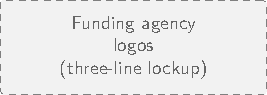
\includegraphics[height=2\coverLogoHeight]{img/funding.pdf}
\end{center}
\vspace{\stretch{1}}

\noindent
\begin{tabular}{@{}p{0.20\textwidth}p{0.76\textwidth}@{}}
	\textit{Keywords:}       & \thesisKeywords\\[\medskipamount]
	\textit{Palabras clave:} & \foreignlanguage{spanish}{\thesisKeywordsES}\\[\medskipamount]
	\textit{Printed by:}    & \thesisPrintedBy\\[\medskipamount]
	\textit{Front \& back:} & \thesisCoverArt\\[\medskipamount]
	\textit{Funding:}       & \thesisGrants\\
\end{tabular}

\vspace{2\bigskipamount}

\noindent Copyright \textcopyright\ \thesisDate\ by \thesisAuthor. This work is licensed under \href{https://creativecommons.org/licenses/by-nc/4.0/}{CC BY-NC 4.0}.

\medskip
\noindent An electronic version of this Thesis is available at
\href{https://example.org}{example.org}.

\medskip
\noindent{\footnotesize Revised: \today}

\end{titlingpage}
\end{document}
